%Version 3.1 December 2024
% See section 11 of the User Manual for version history
%
%%%%%%%%%%%%%%%%%%%%%%%%%%%%%%%%%%%%%%%%%%%%%%%%%%%%%%%%%%%%%%%%%%%%%%
%%                                                                 %%
%% Please do not use \input{...} to include other tex files.       %%
%% Submit your LaTeX manuscript as one .tex document.              %%
%%                                                                 %%
%% All additional figures and files should be attached             %%
%% separately and not embedded in the \TeX\ document itself.       %%
%%                                                                 %%
%%%%%%%%%%%%%%%%%%%%%%%%%%%%%%%%%%%%%%%%%%%%%%%%%%%%%%%%%%%%%%%%%%%%%

%%\documentclass[referee,sn-basic]{sn-jnl}% referee option is meant for double line spacing

%%=======================================================%%
%% to print line numbers in the margin use lineno option %%
%%=======================================================%%

%%\documentclass[lineno,pdflatex,sn-basic]{sn-jnl}% Basic Springer Nature Reference Style/Chemistry Reference Style

%%=========================================================================================%%
%% the documentclass is set to pdflatex as default. You can delete it if not appropriate.  %%
%%=========================================================================================%%

%%\documentclass[sn-basic]{sn-jnl}% Basic Springer Nature Reference Style/Chemistry Reference Style

%%Note: the following reference styles support Namedate and Numbered referencing. By default the style follows the most common style. To switch between the options you can add or remove “Numbered” in the optional parenthesis. 
%%The option is available for: sn-basic.bst, sn-chicago.bst%  
 
%%\documentclass[pdflatex,sn-nature]{sn-jnl}% Style for submissions to Nature Portfolio journals
%%\documentclass[pdflatex,sn-basic]{sn-jnl}% Basic Springer Nature Reference Style/Chemistry Reference Style
\documentclass[pdflatex,sn-mathphys-num]{sn-jnl}% Math and Physical Sciences Numbered Reference Style
%%\documentclass[pdflatex,sn-mathphys-ay]{sn-jnl}% Math and Physical Sciences Author Year Reference Style
%%\documentclass[pdflatex,sn-aps]{sn-jnl}% American Physical Society (APS) Reference Style
%%\documentclass[pdflatex,sn-vancouver-num]{sn-jnl}% Vancouver Numbered Reference Style
%%\documentclass[pdflatex,sn-vancouver-ay]{sn-jnl}% Vancouver Author Year Reference Style
%%\documentclass[pdflatex,sn-apa]{sn-jnl}% APA Reference Style
%%\documentclass[pdflatex,sn-chicago]{sn-jnl}% Chicago-based Humanities Reference Style

%%%% Standard Packages
%%<additional latex packages if required can be included here>

\usepackage{graphicx}%
\usepackage{multirow}%
\usepackage{amsmath,amssymb,amsfonts}%
\usepackage{amsthm}%
\usepackage{mathrsfs}%
\usepackage[title]{appendix}%
\usepackage{xcolor}%
\usepackage{textcomp}%
\usepackage{manyfoot}%
\usepackage{booktabs}%
\usepackage{listings}%
%%%%
\usepackage{xspace}
\usepackage{wrapfig}
\usepackage{capt-of}
\usepackage{tcolorbox}

\newcommand{\eg}{\textit{e.g., }}
\newcommand{\ie}{\textit{i.e., }}

\newcommand{\n}{\texttt{PALACE}\xspace}

%%%%%=============================================================================%%%%
%%%%  Remarks: This template is provided to aid authors with the preparation
%%%%  of original research articles intended for submission to journals published 
%%%%  by Springer Nature. The guidance has been prepared in partnership with 
%%%%  production teams to conform to Springer Nature technical requirements. 
%%%%  Editorial and presentation requirements differ among journal portfolios and 
%%%%  research disciplines. You may find sections in this template are irrelevant 
%%%%  to your work and are empowered to omit any such section if allowed by the 
%%%%  journal you intend to submit to. The submission guidelines and policies 
%%%%  of the journal take precedence. A detailed User Manual is available in the 
%%%%  template package for technical guidance.
%%%%%=============================================================================%%%%

%% as per the requirement new theorem styles can be included as shown below
\theoremstyle{thmstyleone}%
\newtheorem{theorem}{Theorem}%  meant for continuous numbers
%%\newtheorem{theorem}{Theorem}[section]% meant for sectionwise numbers
%% optional argument [theorem] produces theorem numbering sequence instead of independent numbers for Proposition
\newtheorem{proposition}[theorem]{Proposition}% 
%%\newtheorem{proposition}{Proposition}% to get separate numbers for theorem and proposition etc.

\theoremstyle{thmstyletwo}%
\newtheorem{example}{Example}%
\newtheorem{remark}{Remark}%

\theoremstyle{thmstylethree}%
\newtheorem{definition}{Definition}%

\raggedbottom
%%\unnumbered% uncomment this for unnumbered level heads

\begin{document}

\title[Auditing Hidden Reasoning Charges in Commercial LLM APIs through Token-Usage Prediction]{Auditing Hidden Reasoning Charges in Commercial LLM APIs through Token-Usage Prediction}

%%=============================================================%%
%% GivenName	-> \fnm{Joergen W.}
%% Particle	-> \spfx{van der} -> surname prefix
%% FamilyName	-> \sur{Ploeg}
%% Suffix	-> \sfx{IV}
%% \author*[1,2]{\fnm{Joergen W.} \spfx{van der} \sur{Ploeg} 
%%  \sfx{IV}}\email{iauthor@gmail.com}
%%=============================================================%%

\author[1]{\fnm{Ziyao} \sur{Wang}}\email{ziyaow@umd.edu}
\equalcont{These authors contributed equally to this work.}

\author[1]{\fnm{Guoheng} \sur{Sun}}\email{ghsun@umd.edu}
\equalcont{These authors contributed equally to this work.}

\author[1]{\fnm{Yexiao} \sur{He}}\email{yexiaohe@umd.edu}
% \equalcont{These authors contributed equally to this work.}

\author[1]{\fnm{Zheyu} \sur{Shen}}\email{zyshen@umd.edu}
% \equalcont{These authors contributed equally to this work.}

\author[1]{\fnm{Bowei} \sur{Tian}}\email{boweitian@umd.edu}
% \equalcont{These authors contributed equally to this work.}

\author*[1]{\fnm{Ang} \sur{Li}}\email{angliece@umd.edu}
% \equalcont{These authors contributed equally to this work.}

\affil[1]{\orgname{University of Maryland}, \orgaddress{\city{College Park}, \state{Maryland}, \country{USA}}}

% \affil[2]{\orgdiv{Department}, \orgname{Organization}, \orgaddress{\street{Street}, \city{City}, \postcode{10587}, \state{State}, \country{Country}}}

% \affil[3]{\orgdiv{Department}, \orgname{Organization}, \orgaddress{\street{Street}, \city{City}, \postcode{610101}, \state{State}, \country{Country}}}

%%==================================%%
%% Sample for unstructured abstract %%
%%==================================%%

\abstract{Commercial large language model services often hide their internal reasoning traces while charging users for all generated tokens, including hidden reasoning tokens. This makes it difficult for users to audit reported token usage and raises concerns about token inflation and overbilling. However, auditing hidden token usage is challenging because service providers control the full inference process, while reasoning length varies substantially across tasks and prompts. Here we study whether hidden reasoning token counts can be estimated from the prompt and final answer alone. We develop a user-side predictive auditing approach, referred to as PALACE, that is trained to account for differences across reasoning domains. Experiments on mathematical, coding, medical and general reasoning benchmarks show that hidden token counts can be predicted with low relative error and that the resulting estimates can be used to identify simulated token inflation. Across four reasoning domains, PALACE detected 92.9\% of simulated 30\% overreporting events in batches of 50 requests, with a 4.9\% false-positive rate. These results show that predictive auditing can give users an independent way to check reported hidden reasoning token usage without access to internal reasoning traces.}

%%================================%%
%% Sample for structured abstract %%
%%================================%%

% \abstract{\textbf{Purpose:} The abstract serves both as a general introduction to the topic and as a brief, non-technical summary of the main results and their implications. The abstract must not include subheadings (unless expressly permitted in the journal's Instructions to Authors), equations or citations. As a guide the abstract should not exceed 200 words. Most journals do not set a hard limit however authors are advised to check the author instructions for the journal they are submitting to.
% 
% \textbf{Methods:} The abstract serves both as a general introduction to the topic and as a brief, non-technical summary of the main results and their implications. The abstract must not include subheadings (unless expressly permitted in the journal's Instructions to Authors), equations or citations. As a guide the abstract should not exceed 200 words. Most journals do not set a hard limit however authors are advised to check the author instructions for the journal they are submitting to.
% 
% \textbf{Results:} The abstract serves both as a general introduction to the topic and as a brief, non-technical summary of the main results and their implications. The abstract must not include subheadings (unless expressly permitted in the journal's Instructions to Authors), equations or citations. As a guide the abstract should not exceed 200 words. Most journals do not set a hard limit however authors are advised to check the author instructions for the journal they are submitting to.
% 
% \textbf{Conclusion:} The abstract serves both as a general introduction to the topic and as a brief, non-technical summary of the main results and their implications. The abstract must not include subheadings (unless expressly permitted in the journal's Instructions to Authors), equations or citations. As a guide the abstract should not exceed 200 words. Most journals do not set a hard limit however authors are advised to check the author instructions for the journal they are submitting to.}

\keywords{Large language model, Reasoning, Auditing}

%%\pacs[JEL Classification]{D8, H51}

%%\pacs[MSC Classification]{35A01, 65L10, 65L12, 65L20, 65L70}

\setcounter{secnumdepth}{0}

\maketitle

\section{Introduction}

Large language models (LLMs) increasingly rely on extended internal computation to support multi-step reasoning~\citep{guo2025deepseek}, external tool use~\citep{chen2024huatuogpto1medicalcomplexreasoning, zhuang2023toolqa}, and agent coordination~\citep{zhao2024expel}. Such capabilities substantially improve model performance, but they may also generate long intermediate traces containing backtracking steps, exploratory branches, and other verbose content~\citep{aggarwal2025l1}. These reasoning traces are often unnecessary for end users and may expose proprietary model behaviors, system prompts, or agent workflows.

To protect model security and intellectual property, commercial providers such as OpenAI~\citep{openai2025reasoning}, Google~\citep{google2025thinking}, and Anthropic typically do not reveal the complete internal traces produced during reasoning or tool execution. Users may nevertheless be charged for the associated internal tokens in addition to the visible response. Services with this property have been described as \textit{Commercial Opaque LLM Services} (COLS)~\citep{sun2025invisible}. Figure~\ref{fig:problem} illustrates the transparency concern of COLS, where users can observe the final answer but cannot directly verify the hidden reasoning-token usage.

\begin{figure}[!htbp]
    \centering
    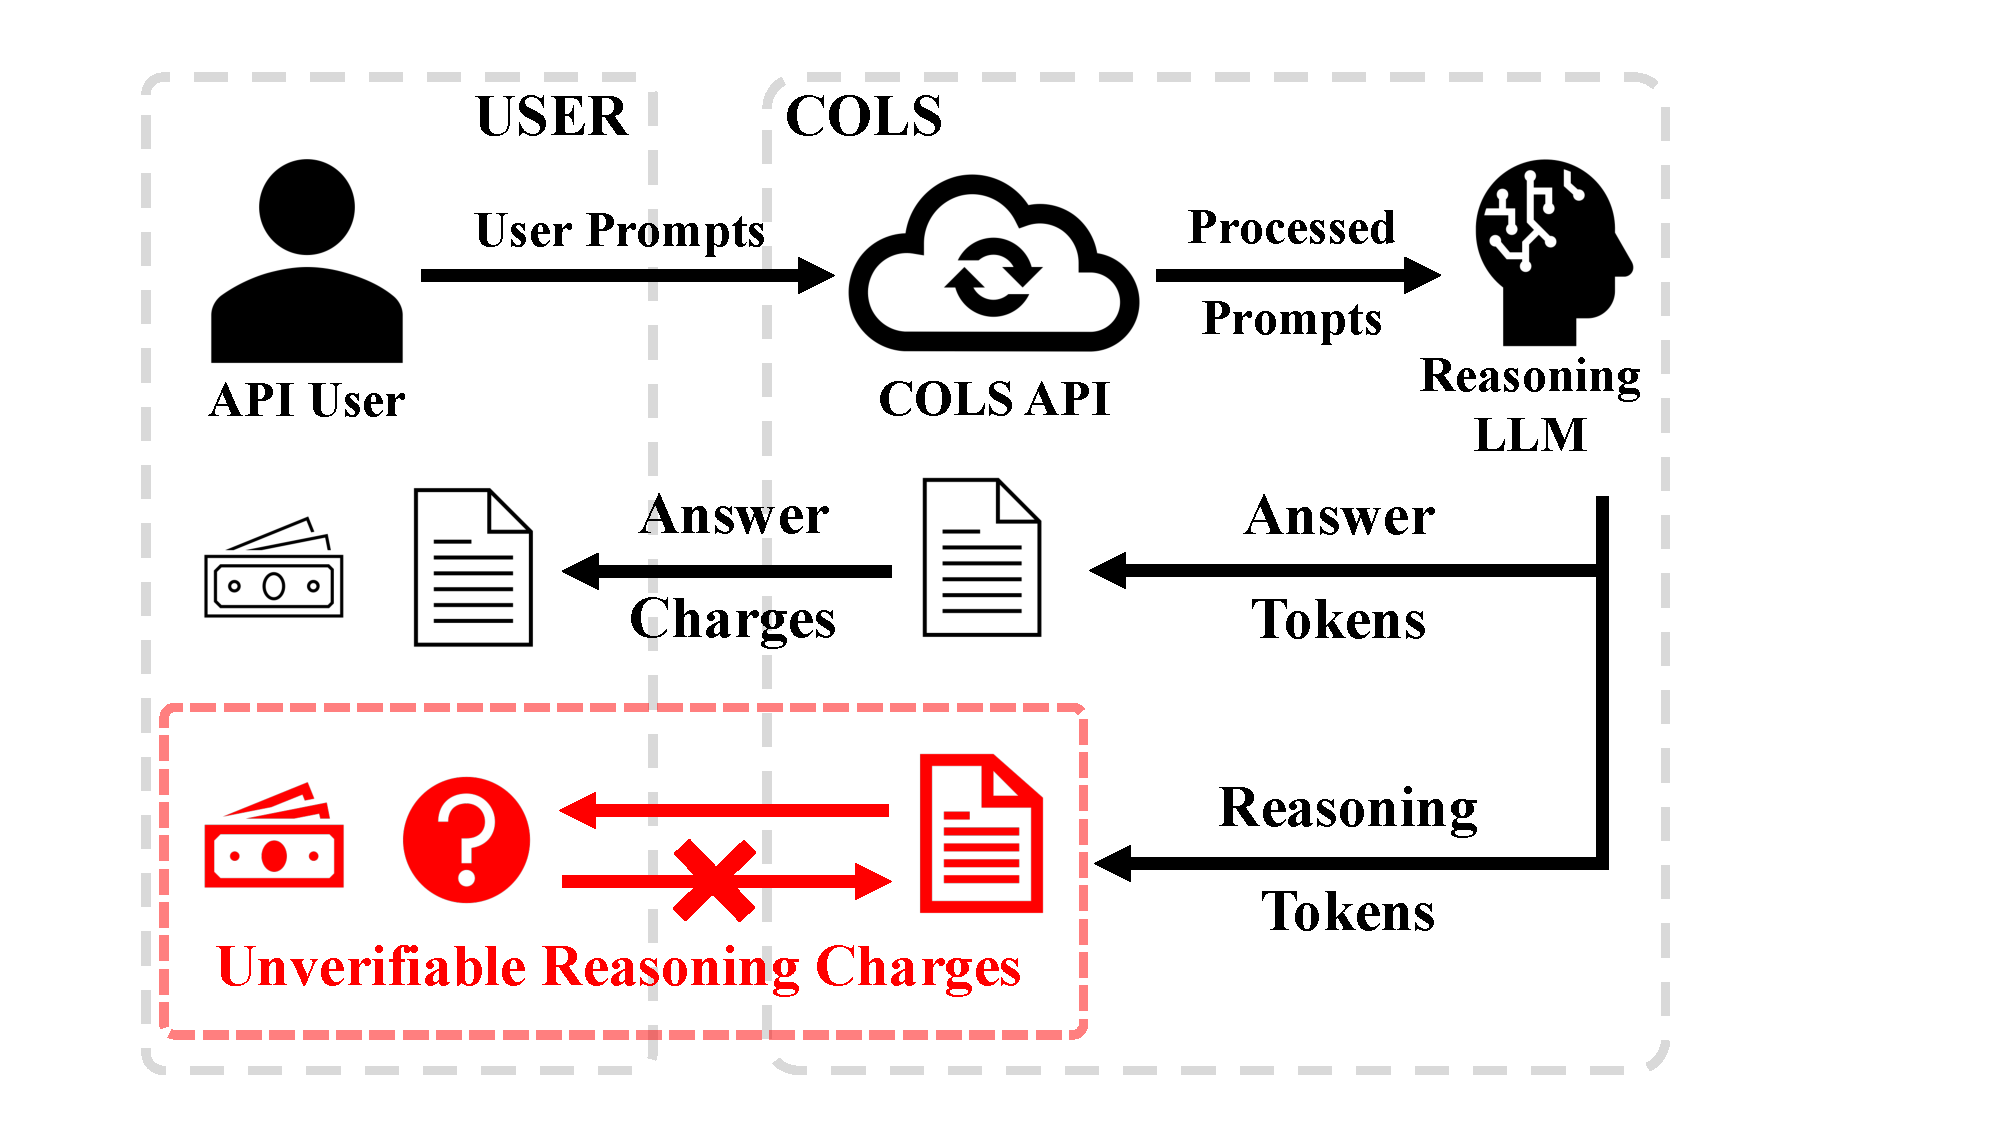
\includegraphics[width=0.70\linewidth]{Figures/intro.pdf}
    \par\smallskip\textbf{Figure~\ref{fig:problem}}\par
\end{figure}

This opaque design raises notable transparency gaps: \textbf{users are charged for token usage they cannot observe or verify}. All token consumption is reported solely by the service provider, whose financial incentives may conflict with those of the user. This creates the risk of \textit{token inflation}, where COLS may over-report token usage to increase billing. 
Empirical studies show that in many state-of-the-art models, over 90\% of tokens are consumed in hidden reasoning, with only a small portion forming the final answer~\citep{sun2025coin}. Even minor inflation under such conditions can lead to considerable increases in expenses, particularly for large-scale API users engaged in synthetic data generation, annotation, or document processing. 
For example, an ARC-AGI run with OpenAI's o3 model consumed 111 million tokens at a cost of \$66,772~\citep{chollet2025o3}, with over 60\% from hidden reasoning tokens. Although there is no evidence of inflation in COLS, the large monetary amounts involved mean that users have legitimate reasons to expect clearer auditing mechanisms, highlighting the need for greater transparency in LLM services. Existing work on auditing commercial LLM services has primarily considered either service-quality substitution or direct verification of reported execution. For quality downgrade, prior studies detect whether a provider silently substitutes a smaller model or a cheaper execution pipeline using output-based statistical tests, benchmark comparisons, log-probability analysis, or trusted execution environments~\citep{cai2025you,yuan2025trust,nvidia2023confidential}. For quantity inflation, CoIn~\citep{sun2025coin} constructs a hash-tree-based mechanism that allows an auditor to verify token counts and semantic consistency through
additional interaction with the service provider.

Auditing token usage under these conditions is challenging for two reasons. First, cryptographic approaches~\citep{sun2025coin} require the auditor to access hidden reasoning traces in order to perform verification. In practice, however, the entire reasoning process is controlled by the COLS, making such methods impractical. Second, user-side heuristics based on input–output lengths are unreliable, because reasoning token usage varies drastically with domain, prompt style, and task complexity~\citep{jin2024impact}. Together, these challenges create a critical need for \textbf{an auditing solution that works without access to hidden traces and remains robust to reasoning variability}.

% \begin{figure}[t]
%     \centering
%     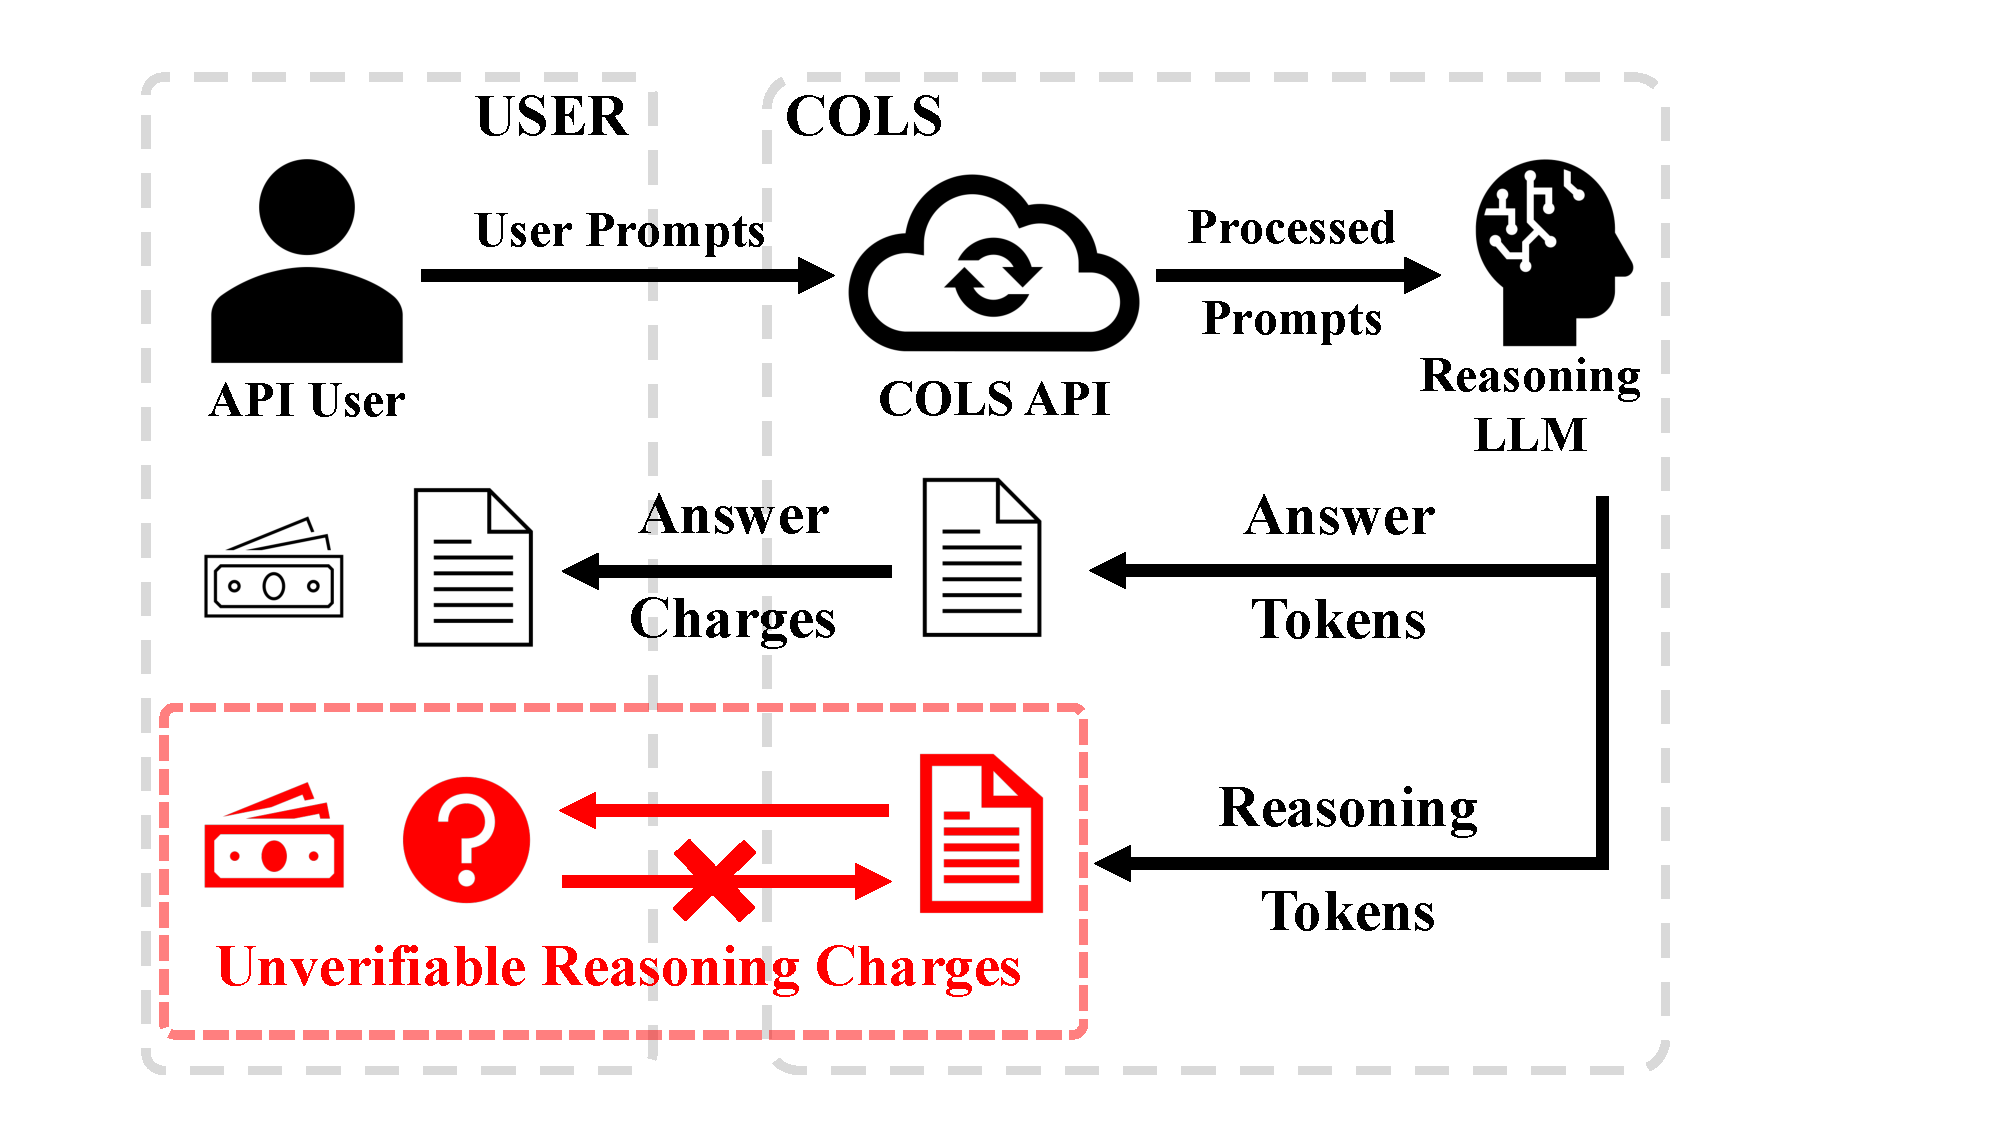
\includegraphics[width=0.47\textwidth]{Figures/intro.pdf}
%     \caption{The transparency concern of COLS.}
%     \label{fig:problem}
% \end{figure}

To address these challenges, we introduce {\n} (\textit{Predictive Auditing of LLM APIs via Reasoning Token Count Estimation}), a user-side framework that statistically estimates hidden
reasoning-token usage from observable prompt-answer pairs. Rather than
attempting to verify the exact reasoning token number,
{\n} provides an independent estimate of the token usage expected under the
audited model configuration. Provider-reported usage can then be compared with
these estimates at both the request and aggregate levels to identify
statistically unusual or systematic discrepancies.
Because no user-side method can directly recover fully hidden computation
without any information from the provider, we adopt a limited cooperation
assumption. Specifically, the provider releases a small auxiliary dataset
attributed to the audited model configuration, where each sample contains a
prompt, its associated reasoning trace, and the final answer. This dataset is
used to calibrate the auditor. Once calibrated, {\n} does not require access to
the internal traces or intermediate representations of the queries being
audited, nor does it require additional interaction with the service during
auditing.

{\n} estimates reasoning-token usage by learning the relationship between the
observable semantics of a prompt-answer pair and the length of its hidden
reasoning process. To account for the substantial variation across tasks and
domains, the framework combines domain-specific adaptation based on Group
Relative Policy Optimization (GRPO)~\citep{shao2024deepseekmath} with a
lightweight router that selects the appropriate prediction module for each
query. Given a prompt, the corresponding response returned by the service, and
the relevant API configuration, {\n} produces an estimated hidden-token count.
The resulting estimates support two complementary forms of auditing. At the
request level, they provide a reference for assessing whether reported usage is
consistent with the expected range for a particular interaction. At the
aggregate level, estimates from multiple requests can be combined to reveal
systematic discrepancies that may not be distinguishable from ordinary
prediction error in any single request.

% \textit{\textbf{Our aim is not to overstate the issue or to imply that COLS overcharge users, but to suggest that COLS offer auxiliary datasets to enable real-time auditing, strengthen trust, and enhance providers’ reputations.}} 
Our main contributions are summarized as follows:
\begin{itemize}
    \item We formulate reasoning-length estimation as a basis for user-side auditing of hidden reasoning-token usage in commercial opaque LLM services.

    \item We develop {\n}, which combines GRPO-based domain adaptation with a lightweight router to estimate hidden reasoning length directly from observable prompt--answer pairs, without requiring access to the internal execution traces of the queries being audited.

    \item We construct multi-domain benchmark datasets covering mathematical, coding, medical, and general reasoning tasks, and show that {\n} achieves low relative estimation error and stable aggregate estimates across domains, supporting request-level cost assessment and the detection of systematic reporting discrepancies.
\end{itemize}


\begin{table*}[t]
\caption{Prediction accuracy and error of {\n}. The upper block reports Pass@1/Pass@5 accuracy (\%), and the lower block reports Average (AVG.) and Aggregated (AGG.) errors. CoIn reports the detection rate at a fixed token-injection rate. Pass@1 and Pass@5 are prediction metrics.}
\label{tab:acc_err}
\centering
\footnotesize
\resizebox{\textwidth}{!}{
\begin{tabular}{cc|cc|cc|cc|cc}
\toprule
\textbf{Model} & \textbf{Method} 
& \multicolumn{2}{c}{\textbf{General}} 
& \multicolumn{2}{c}{\textbf{Math}} 
& \multicolumn{2}{c}{\textbf{Coding}} 
& \multicolumn{2}{c}{\textbf{Medical}} \\
& & \textbf{Pass@1} & \textbf{Pass@5} & \textbf{Pass@1} & \textbf{Pass@5} & \textbf{Pass@1} & \textbf{Pass@5} & \textbf{Pass@1} & \textbf{Pass@5} \\
\midrule
& \textbf{CoIn (Detection rate)} &63.21&---&44.22&---&38.12&---&46.25&---\\
& \textbf{MLP} & 67.86 & 67.89 & 27.11 & 32.87 & 44.95 & 47.77 & 44.99 & 51.04 \\
\midrule
\multirow{2}{*}{\textbf{Qwen2.5-3B}} 
& \textbf{LoRA} & 85.95 & 96.74 & 58.56 & 82.79 & 52.92 & 82.69 & 50.25 & 84.87 \\
& \textbf{PALACE} &\textbf{87.28}&88.50&\textbf{62.37}&67.15&\textbf{59.91}&64.36&\textbf{59.13}&62.39 \\
\midrule
\multirow{2}{*}{\textbf{Qwen2.5-1.5B}}
& \textbf{LoRA} &85.66&94.07&49.26&84.47& 35.81 & 81.21 & 51.93 & 83.88 \\
& \textbf{PALACE} & \textbf{88.40} &88.65& \textbf{63.81} &65.44& \textbf{58.39} &59.51& \textbf{59.71} & 62.86\\
\midrule
\multirow{2}{*}{\textbf{LLaMA3.2-3B}}
& \textbf{LoRA} &62.74&89.59&32.53&59.08&36.40&53.31&36.99&60.64\\
& \textbf{PALACE} &\textbf{81.42}&86.86&\textbf{51.73}&65.60&\textbf{65.27}&71.15&\textbf{59.59}&66.68\\
\midrule
\multirow{2}{*}{\textbf{LLaMA3.2-1B}}
& \textbf{LoRA} &65.48&82.10&24.34&71.72&\textbf{35.21}&54.50&37.39&56.38\\
& \textbf{PALACE} &\textbf{79.42}&83.51&\textbf{43.48}&53.95&34.25&44.00&\textbf{43.36}&50.13\\
\midrule
\midrule
& & \textbf{AVG($\downarrow$)} & \textbf{AGG($\downarrow$)} & \textbf{AVG($\downarrow$)} & \textbf{AGG($\downarrow$)} & \textbf{AVG($\downarrow$)} & \textbf{AGG($\downarrow$)} & \textbf{AVG($\downarrow$)} & \textbf{AGG($\downarrow$)} \\
\midrule
& \textbf{MLP} & 26.39 & 1.25 & 87.45 & 2.24 &87.44 &1.47 & 79.02 & 1.41 \\
\midrule
\multirow{2}{*}{\textbf{Qwen2.5-3B}}
& \textbf{LoRA} & 18.11 & 3.93 & 40.67 & 8.74 & 40.34 & 4.07 & 39.69 & 18.24 \\
& \textbf{PALACE} &\textbf{17.82}&6.34&\textbf{30.58}&6.67&\textbf{34.76}&5.61&\textbf{34.09}&13.56\\
\midrule
\multirow{2}{*}{\textbf{Qwen2.5-1.5B}}
& \textbf{LoRA} &19.03&5.80&58.63&2.43& 64.61 & 1.86 & 35.82 & 33.31 \\
& \textbf{PALACE} & \textbf{18.43} & 4.80 & \textbf{36.48} & 6.72 & \textbf{48.46} & 7.75 & \textbf{33.60} & 16.68 \\
\midrule
\multirow{2}{*}{\textbf{LLaMA3.2-3B}}
& \textbf{LoRA} &25.23&8.34&30.57&11.80&64.71&2.32&51.49&17.02\\
& \textbf{PALACE} &\textbf{18.09}&5.67&\textbf{29.19}&10.42&\textbf{29.43}&12.78&\textbf{29.68}&23.65\\
\midrule
\multirow{2}{*}{\textbf{LLaMA3.2-1B}}
& \textbf{LoRA} &30.37&10.20&58.41&37.19&52.88&32.11&50.89&27.61\\
& \textbf{PALACE} &\textbf{21.65}&16.84&\textbf{56.98}&15.71&\textbf{52.74}&38.67&\textbf{40.62}&55.82\\
\bottomrule
\end{tabular}}
\vspace{-2mm}
\end{table*}

\section{Results}

\subsection{Predicting hidden reasoning-token usage}

Table~\ref{tab:acc_err} demonstrates that {\n} achieves the strongest
overall Pass@1 prediction performance across most domains and model sizes. By leveraging semantic information rather than relying solely on text length and utilizing the reasoning abilities of the auditing model, {\n} consistently delivers high Pass@1 accuracy, even on reasoning-heavy tasks like mathematics. For instance, {\n} predicts the reasoning length with 63.81\% accuracy under the 33\% relative error, while baselines cannot exceed even 50\% accuracy in the same setting.
LoRA fine-tuning achieves higher Pass@5 in most Table~\ref{tab:acc_err} comparisons. Pass@5 measures whether at least one of five samples falls within the prediction tolerance, and the detection experiments use a single greedy prediction.

For CoIn, Table~\ref{tab:acc_err} reports the fraction of injected samples correctly flagged at a fixed token-injection rate.

On the held-out split, PALACE achieved 68.6\% Pass@33 across four domains, compared with 54.8\% for per-domain LightGBM using length and surface features and 49.1\% for the two-length MLP. With the same backbone, training data, and input--output format, full-parameter SFT achieved \(72.2\% \pm 0.7\%\) across three seeds. These results show the value of using prompt and answer content and establish supervised fine-tuning as another effective way to train the auditor.

Simple baselines can achieve low aggregate error by predicting close to the dataset mean for many requests. Their predictions add up to a reasonable total, but miss how much reasoning-token usage varies from one request to another. PALACE reduces average error on individual requests while keeping aggregate error low, so its estimates are useful both for individual requests and for the workload as a whole.

\subsection{Auto-Regressive Model and Task Router improves heterogeneous prediction}


\begin{wrapfigure}{r}{0.46\textwidth}
\centering
\footnotesize
\setlength{\tabcolsep}{4pt}
\renewcommand{\arraystretch}{1.08}

\captionof{table}{\textbf{Regression vs.\ classification.} Classification accuracy is the percentage of predictions that match the reference token-count bucket. Regression accuracy is Pass@1 at a 33\% relative error tolerance.}
\label{tab:tree}

\begin{tabular}{@{}llcc@{}}
\toprule
\textbf{Model}
&
\textbf{Dataset}
&
\textbf{Class.}
&
\textbf{Reg.}
\\
\midrule

\multirow{4}{*}{Qwen2.5-3B}
& General & 62.15 & \textbf{87.28} \\
& Math    & 56.02 & \textbf{62.37} \\
& Coding  & 43.44 & \textbf{59.91} \\
& Medical & 52.10 & \textbf{59.13} \\

\midrule

\multirow{4}{*}{Qwen2.5-1.5B}
& General & 71.34 & \textbf{88.40} \\
& Math    & 55.27 & \textbf{63.81} \\
& Coding  & 51.02 & \textbf{58.39} \\
& Medical & 49.83 & \textbf{59.71} \\

\bottomrule
\end{tabular}

\vspace{-15pt}
\end{wrapfigure}
We further examined whether a classification LLM could serve as an alternative to {\n}’s regression‑based token estimation. In the classification setting, reasoning token counts are discretized into usage buckets and the model predicts the corresponding class rather than the exact number. This design allows training by simply attaching a classification head.
However, as shown in Table \ref{tab:tree}, the classification approach lags behind {\n}’s GRPO across almost every dataset. On Qwen2.5‑3B, classification achieves reasonable performance (\eg 62.15 on the General set), but remains notably lower than {\n}’s 87.28. Similar gaps are seen in all other domains. The trend is consistent on the smaller Qwen2.5‑1.5B model.
% These results suggest that although the accuracy of classification models is not computed in exactly the same way as regression, the data show a clear gap between classification and regression, especially GRPO based regression. A likely reason is that classification does not fully leverage the LLM’s reasoning ability, which leads to weaker token count estimation. The details of classification dataset construction are provided in the
% Supplementary Information.

\par
\WFclear

% \begin{table}[t]
% \caption{Regression vs classification.}
% 	\label{tab_tree}
% 	\centering
% 	\footnotesize
%         \resizebox{2.9in}{!}{
% 	\begin{tabular}{c|c|cc}
% 		\toprule
% \textbf{Models} &\textbf{Dataset} &{\textbf{Classification}}&\textbf{{\n}} \\
%         \midrule
%         \multirow{4}{*}{\textbf{Qwen2.5-3B}}&\textbf{General}&62.15&\textbf{87.28}\\
%         &\textbf{Math}&56.02&\textbf{62.37}\\
%         &\textbf{Coding}&43.44&\textbf{59.91}\\
%         &\textbf{Medical}&52.10&\textbf{59.13}\\
%         \midrule
%         \multirow{4}{*}{\textbf{Qwen2.5-1.5B}}&\textbf{General}&71.34&\textbf{88.40}\\
%         &\textbf{Math}&55.27&\textbf{63.81}\\
%         &\textbf{Coding}&51.02&\textbf{58.39}\\
%         &\textbf{Medical}&49.83&\textbf{59.71}\\
% 		\bottomrule
% 	\end{tabular}}
%     \vspace{-0.1cm}
% \end{table}
To assess whether routing truly improves auditing performance, we compared {\n}’s router-based design with a simpler \textit{merged dataset} baseline, where all domain data were combined and a single GRPO adapter was trained across tasks. As shown in Figure \ref{fig:general_compare}, the router consistently yields stronger results on Qwen2.5‑1.5B. It achieves higher Pass@1 accuracy on nearly every subtask, from General reasoning to Medical queries, and also provides small but meaningful gains on Pass@5. This improvement comes from the router’s ability to partition inputs by domain and activate the most relevant GRPO adapter, instead of forcing one generic adapter to absorb heterogeneous reasoning styles. By doing so, the router helps {\n} mitigate variance across tasks and reduces the cross‑domain interference observed in the merged‑training setup, resulting in more stable and accurate token‑length predictions overall.

\begin{figure}[!htbp]
    \centering
    
\includegraphics[width=1.0\linewidth]{Figures/merged.pdf}
    \par\smallskip\textbf{Figure~\ref{fig:general_compare}}\par
\end{figure}


\subsection{Predictive auditing identifies simulated reporting discrepancies}

Figure~\ref{fig:rateacc} summarizes prediction accuracy across error tolerances for PALACE and LoRA and detection rates across injection rates for CoIn. In a separate simulation, PALACE detected 92.9\% of batches with 30\% overreporting at 50 requests per batch, with a 4.9\% false-positive rate.

\begin{figure}[!htbp]
    \centering
    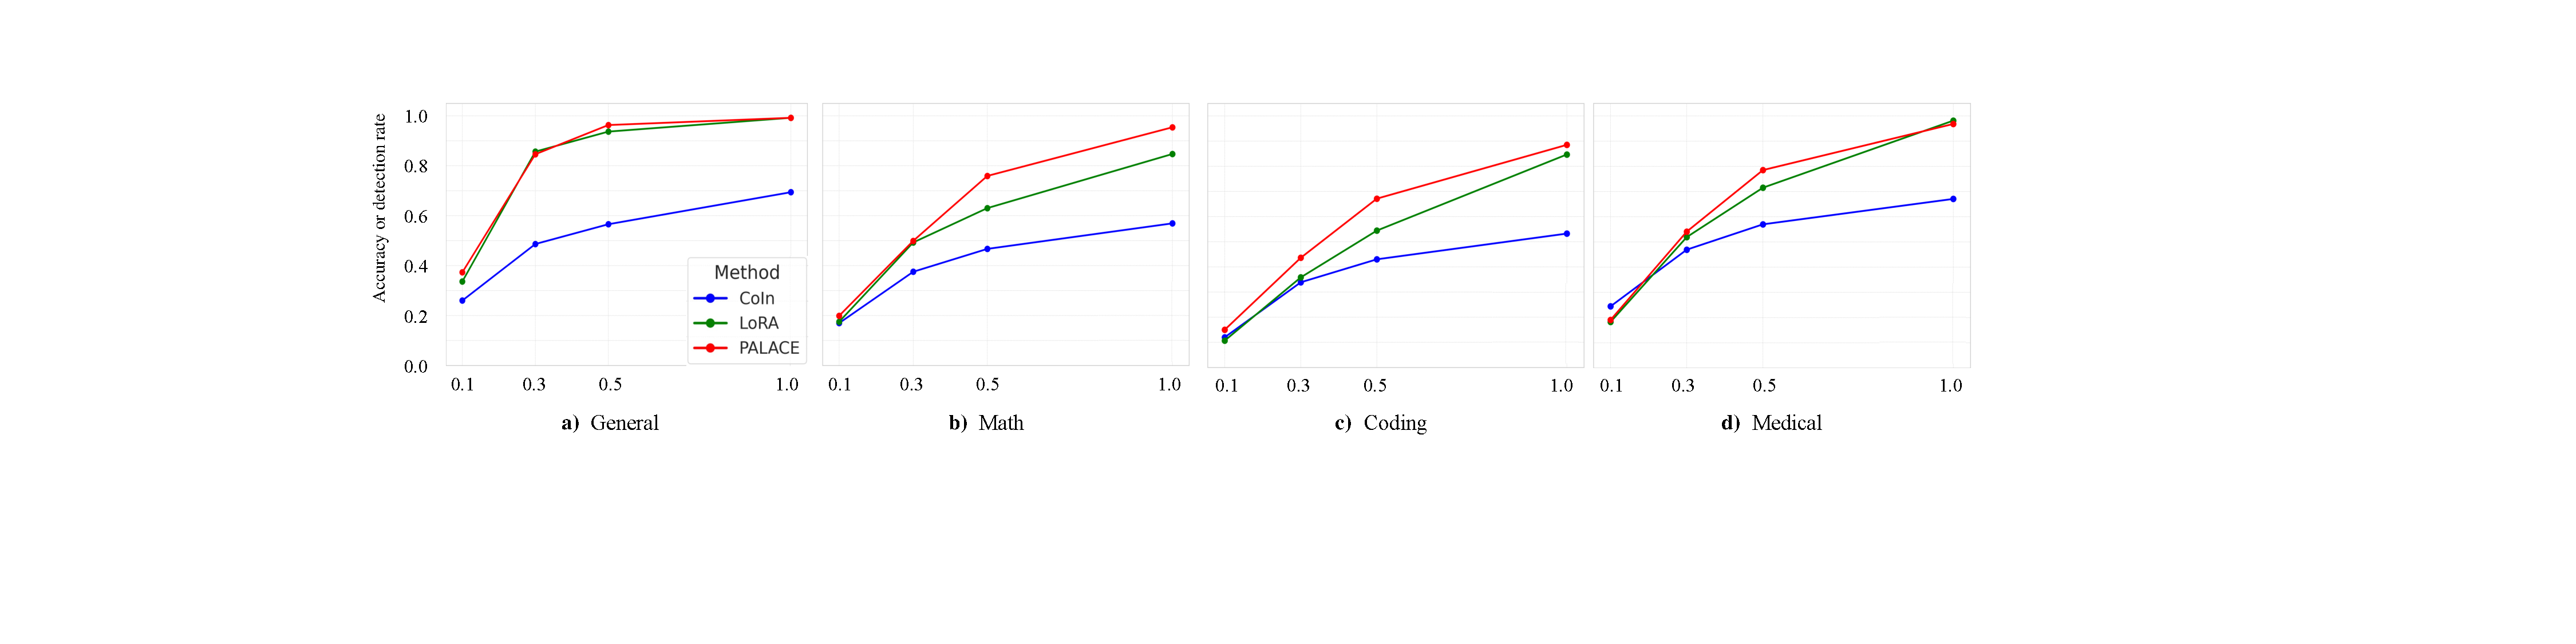
\includegraphics[width=1.0\linewidth]{Figures/error.pdf}
    \par\smallskip\textbf{Figure~\ref{fig:rateacc}}\par
\end{figure}


Figure~\ref{fig:grpo-math-qwen} shows the training reward for the Qwen2.5-3B GRPO auditor over one epoch on 90,000 Math examples. The reward rises early in training and fluctuates around a plateau in the second half of the run.

\begin{figure}[!htbp]
    \centering
    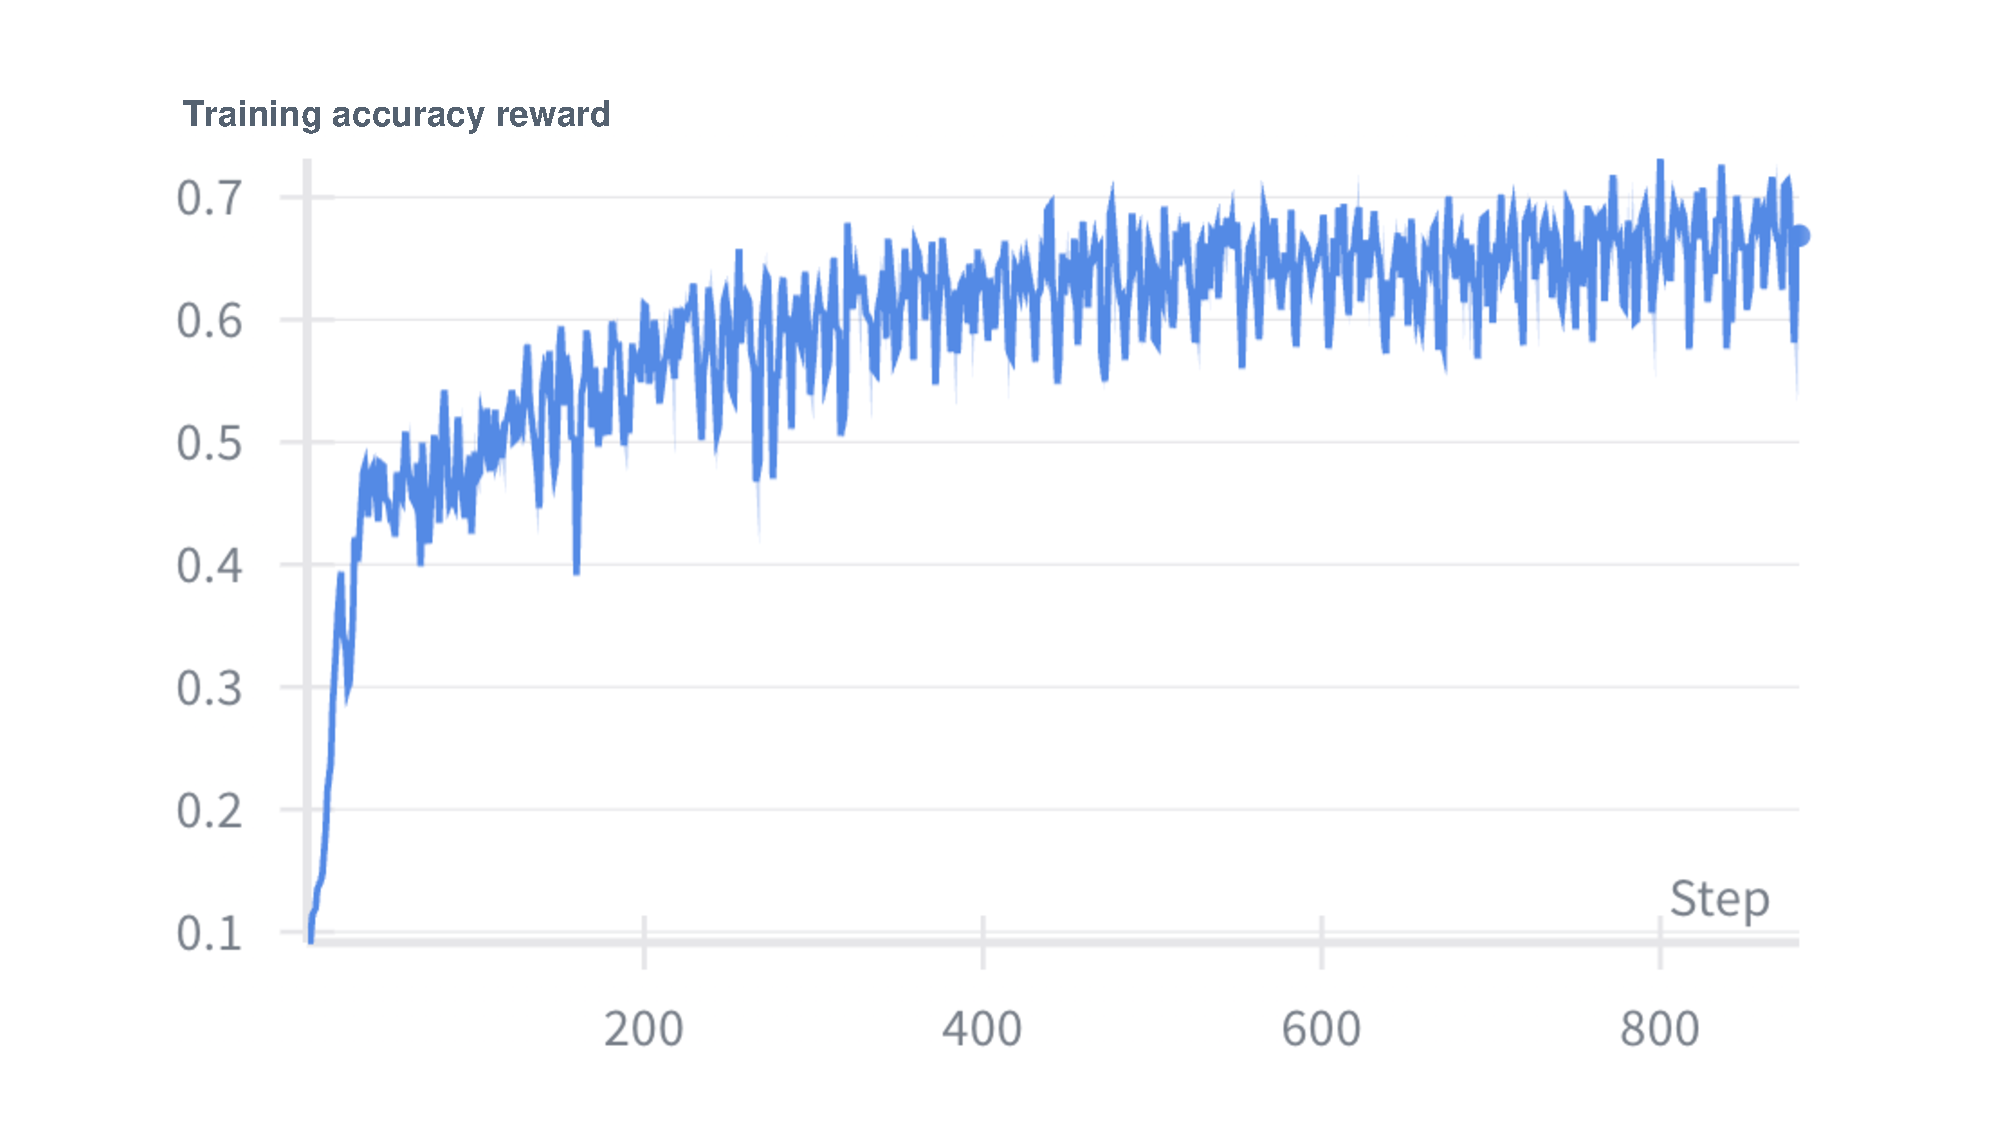
\includegraphics[width=0.75\linewidth]{Figures/grpo_exp.pdf}
    \par\smallskip\textbf{Figure~\ref{fig:grpo-math-qwen}}\par
\end{figure}

\section{Discussion}

This work demonstrates that hidden reasoning-token usage in commercial opaque
LLM services can be estimated from observable prompt--answer pairs. Across
mathematical, coding, medical, and general reasoning tasks, {\n} achieves strong
request-level prediction accuracy while maintaining low average and aggregated
errors. These results indicate that reasoning-token consumption exhibits
learnable patterns rather than depending only on surface-level features such as
prompt and response length.

The comparison with length-based baselines highlights the value of modeling the
prompt and answer text. The matched SFT comparison shows that supervised training
can also produce an accurate auditor. Length-based predictors are
limited to shallow correlations, whereas {\n} reasons over the full
prompt--answer pair before estimating hidden-token usage. The domain-specific
GRPO modules further capture differences among mathematical derivations,
program synthesis, medical diagnosis, and general problem solving. Combined
with the lightweight router, this design reduces interference across
heterogeneous domains and improves prediction consistency compared with
training a single model on merged data.

Individual predictions provide a reference for follow-up, but reasoning lengths vary substantially across requests. At a nominal 5\% false-positive rate, PALACE detected 11.3--36.8\% of individual requests with 30\% overreporting across the four domains. For batches of 50 requests, the detection rate reached 92.9\% with a 4.9\% false-positive rate. This increase shows how aggregating requests makes systematic overreporting easier to detect.

Predictive auditing provides a different deployment trade-off from
cryptographic verification. Cryptographic methods can offer stronger guarantees
but generally require provider-side instrumentation, access to committed
execution records, or changes to the serving infrastructure. In contrast, {\n}
requires only an auxiliary dataset for training and calibration, after which it
can audit prompt--answer pairs without accessing hidden traces or modifying the
service pipeline. The two approaches are therefore complementary: predictive
auditing enables lightweight continuous monitoring, while cryptographic
mechanisms can provide stronger guarantees when deeper provider integration is
available.

Predictive auditing requires trusted reference counts from the audited model and configuration, and changes in model settings or workload mix may require recalibration. When coding requests made up 70\% of the workload, a per-domain calibration correction reduced the false-positive rate for 100-request batches from 25.9\% to 3.5\%. Our evaluation uses open-model traces and simulated overreporting.

Overall, {\n} establishes reasoning-length prediction as an effective foundation
for auditing hidden token usage in opaque LLM services. By combining semantic
reasoning, GRPO-based adaptation, and domain-aware routing, it provides accurate
request-level estimates and stable aggregate predictions, offering a practical
path toward more transparent and auditable commercial LLM services.


\section{Methods}

\begin{figure}[!htbp]
    \centering
    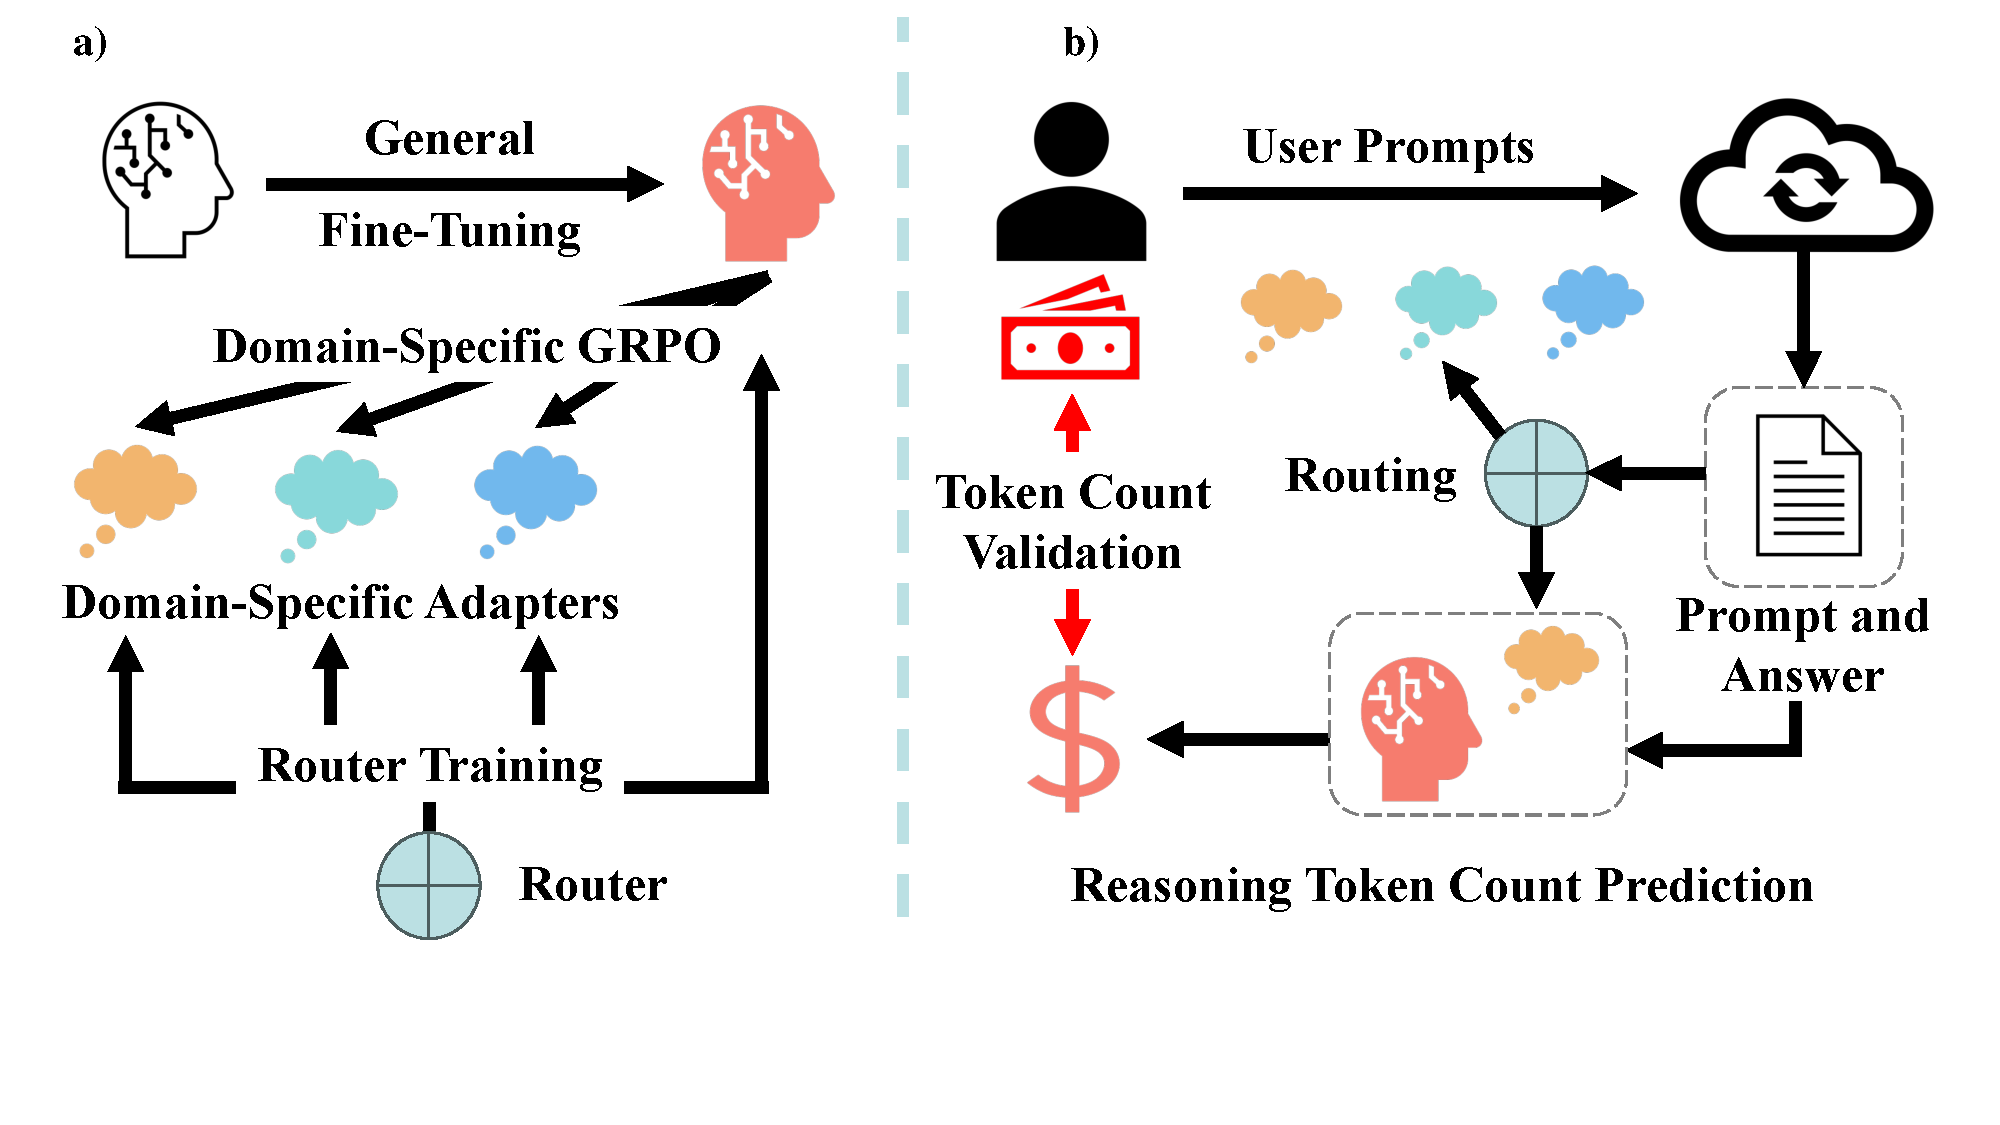
\includegraphics[width=0.95\linewidth]{Figures/workflow.pdf}
    \par\smallskip\textbf{Figure~\ref{fig:workflow}}\par
\end{figure}

\subsection{Dataset Construction}
\label{sec:dataset}

Since prior work does not address auditing the reasoning length based solely on prompt--answer pairs, we construct the first \textit{reasoning length auditing dataset}. Specifically, we curate four datasets comprising multi-step reasoning traces generated by DeepSeek-R1~\citep{guo2025deepseek} and DeepSeek-R1-Distill-Llama-70B. These datasets span diverse domains to support generalization and robust evaluation~\citep{openr1}:

\begin{itemize}
    \item \textbf{OpenR1-Math}: A large-scale dataset for mathematical reasoning, consisting of 220K problems sampled from NuminaMath 1.5. Each question is annotated with 2--4 reasoning traces generated by DeepSeek-R1.

    \item \textbf{OpenR1-Code}: A dataset focused on program synthesis, with samples exhibiting plan-and-execute style reasoning patterns.

    \item \textbf{Medical}: A distilled SFT dataset generated by DeepSeek-R1 (Full Power version), targeting medically verifiable diagnostic questions based on HuatuoGPT-o1.

    \item \textbf{General Reasoning}: A large-scale synthetic dataset containing over 22 million open-domain multi-step QA examples, generated using DeepSeek-R1-Distill-Llama-70B. This dataset provides broad coverage of reasoning styles across domains.
\end{itemize}

We refer to these datasets as $\mathcal{D}_M$, $\mathcal{D}_C$, $\mathcal{D}_{\text{Med}}$, and $\mathcal{D}_G$, respectively.


The GRPO auditing dataset is constructed to train the auditing model under GRPO. Unlike a supervised regression dataset that uses ground-truth labels for direct loss computation, this dataset provides reference values that GRPO converts into reward signals for policy optimization.  
Each sample consists of a structured prompt that includes a \texttt{<Problem>} section providing the user prompt, a \texttt{<Solution>} section showing the response from COLS, and explicit instructions directing the model to generate step-by-step reasoning inside \texttt{<think>} tags and output a predicted token count in JSON format within \texttt{<answer>} tags. To stabilize training and improve estimation accuracy, the prompt also provides auxiliary cues such as prompt and answer token lengths, which correlate with reasoning complexity. This structured setup provides the reference for reward computation, allowing GRPO to refine both the reasoning process and the accuracy of token count predictions across domains. The complete training prompt is provided in Figure~\ref{fig:input_rl}.

\begin{figure}[!htbp]
    \centering
    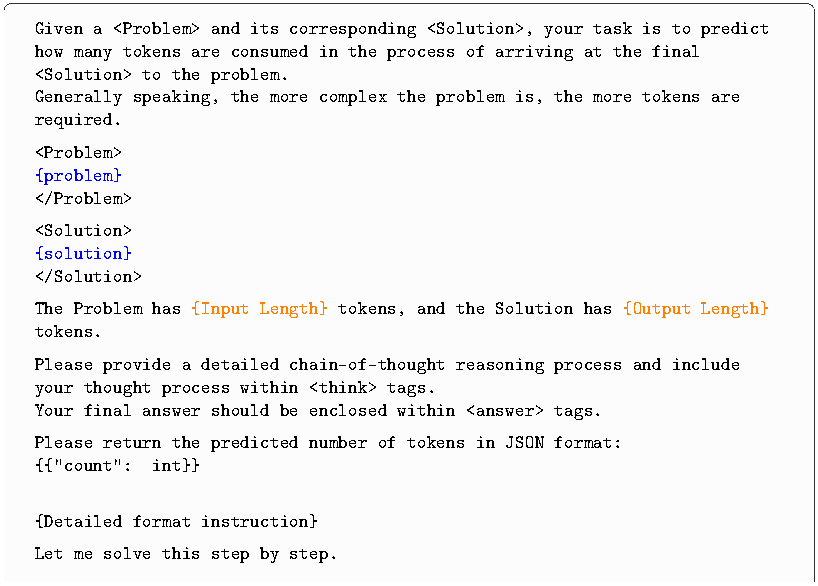
\includegraphics[width=0.91\linewidth]{Figures/figure6.pdf}
    \par\smallskip\textbf{Figure~\ref{fig:input_rl}}\par
\end{figure}

\subsection{Auditing models}

As illustrated in Figure~\ref{fig:workflow}, \n serves as a trusted third-party auditor for commercial LLM services. It begins by acquiring a lightweight auxiliary dataset from the COLS provider and constructing an auditing dataset based on it. A general-purpose auditing model is then obtained by fine-tuning a base LLM on generic QA tasks.
To accommodate diverse reasoning styles across domains and LLM APIs, \n further applies GRPO on domain-specific datasets to derive task-specific parameter deltas, referred to as GRPO-augmented modules. A lightweight router is trained to classify user prompts by domain and select the appropriate GRPO-augmented module for inference.
During auditing, the user submits a prompt and the corresponding COLS output. \n classifies the prompt's domain, loads the relevant GRPO module, and processes the prompt--answer pair using a standardized template. The auditing model then predicts the number of hidden reasoning tokens, expanding this prediction into a tolerance interval. If the predicted token count deviates from the COLS-reported count beyond a threshold, the sample is flagged as potentially inflated. 
%A dataset exhibiting a high proportion of such samples or a large cumulative error suggests inflationary behavior by the COLS.
A dataset exhibiting a high proportion of such samples or a large cumulative error may indicate inflationary behavior by the COLS.

\subsection{GRPO-Augmented LLM Training}
To establish the auditing capability, \n first fine-tunes a base LLM $\mathcal{W}$ on a general QA dataset $\mathcal{D}_G$ to obtain a general-purpose auditing model $\mathcal{W}_G$. This model is trained to estimate hidden reasoning token count required for solving a given problem, based on the problem statement and the final answer:
% Equation placeholder:
\begin{equation}
\mathcal{W}_G = \arg\min_{\mathcal{W}} \; \mathbb{E}_{(x, y) \sim \mathcal{D}_G} \left[ \mathcal{L}_{\mathcal{W}}(x,y) \right].
\end{equation}
Here \(\mathcal{L}_{\mathcal{W}}(x,y)=-T^{-1}\sum_{t=1}^{T}\log p_{\mathcal{W}}(a_t\mid x,a_{<t})\) is the next-token cross-entropy averaged over the \(T\) tokens of the numeric target \(y\). The input \(x\) contains the problem and final answer in the auditor template, and only the target tokens \(a_1,\ldots,a_T\) contribute to the loss.

Because reasoning complexity varies significantly across tasks and models, we further enhance $\mathcal{W}_G$ using GRPO on domain-specific datasets. For each domain \(d\), we perform GRPO on its corresponding dataset \(\mathcal{D}_d\). For coding, this dataset is \(\mathcal{D}_C\). The resulting GRPO-updated model is stored as a domain-specific delta.
We define a reward function that encourages accurate predictions within a relative error threshold $\delta$ and accounts for the underlying reasoning complexity. Let $y$ be the ground-truth hidden reasoning token count and $\hat{y}$ be the predicted reasoning length from auxiliary data. 
The reward is defined as:

\begin{equation}
R(\hat{y}, y) = \max\left(0, 1 - \frac{|\hat{y} - y|}{|y|}\right).
\end{equation}
 
This reward smoothly penalizes prediction error relative to the magnitude of the target value, and is clipped to lie within the $[0, 1]$ interval.


We adopt GRPO~\citep{shao2024deepseekmath} as it has shown strong effectiveness on structured reasoning tasks, making it a natural fit for {\n}. RL is particularly suitable in this setting, because correctness can be directly verified to provide automatic rewards. Formally, let $\pi_\theta$ denote the policy model. For each input $Q$, the model generates $N$ candidate rollouts $\{a_{Q,1},...,a_{Q,N}\}$, each evaluated with explicit rewards. These per-group rollouts yield a \textit{group-wise advantage}, which compares each rollout’s reward to the group average, reducing variance and stabilizing training. The GRPO objective is: 

{\small
\begin{equation}
\begin{aligned}
J_{\text{GRPO}}(\theta)
&= \mathbb{E}\!\left[
\frac{1}{N}\sum_{i=1}^N
\min\!\Big(
r_i A_i,\;
\mathrm{clip}(r_i, 1-\epsilon, 1+\epsilon)A_i
\Big)
\right] \\
&\quad - \beta\, D_{\text{KL}}\!\left(\pi_\theta \,\|\, \pi_{\text{ref}}\right).
\end{aligned}
\end{equation}}
% \begin{equation}  
% J_{\text{GRPO}}(\theta) = \mathbb{E}\!\left[\tfrac{1}{N}\!\sum_{i=1}^N \min\!\Big(r_i A_i,\; \mathrm{clip}(r_i,\,1-\epsilon,\,1+\epsilon)A_i\Big)\right] - \beta D_{\text{KL}}(\pi_\theta \| \pi_{ref}),  
% \end{equation}  
where $r_i=\tfrac{\pi_\theta(a_i|Q)}{\pi_{\theta_{\text{old}}}(a_i|Q)}$ is the likelihood ratio, $A_i$ the group-wise advantage, and $D_{\text{KL}}$ a regularization term against a reference model~\citep{ouyang2022training}.  
Integrated into the adaptation module $\Delta \mathcal{W}_C$, this objective equips {\n} with specialized reasoning-length prediction, improving accuracy on complex tasks.  


\subsection{Router Construction}

To enable domain-aware auditing, we train a lightweight router to classify user prompts into supported domains, enabling dynamic selection of the appropriate GRPO module, thereby improving prediction accuracy while avoiding the need to deploy a large monolithic model.

We denote the router as a classification function \( f_{\text{router}}: x \mapsto d \), where \(x\) is the user prompt and \(d \in \{1, \dots, D\}\) is the domain index corresponding to one of the GRPO-specialized domains. We train \(f_{\text{router}}\) on a small subset of samples selected from each dataset \(\mathcal{D}_M, \mathcal{D}_C, \mathcal{D}_{\text{Med}}, \mathcal{D}_G\), using only the prompt text and its associated domain label.

The objective is a standard cross-entropy loss over the domain labels:
\begin{equation}
\mathcal{L}_{\text{router}} = - \sum_{(x, d) \in \mathcal{D}_{\text{router}}} \log p(d \mid x),
\end{equation}
where \(\mathcal{D}_{\text{router}}\) is the router training set randomly sampled from the domain-specific datasets.
During inference, given a new prompt \(x\), the router first predicts its domain:
\begin{equation}
\hat{d} = f_{\text{router}}(x).
\end{equation}

{\n} loads the corresponding GRPO module \(\Delta \mathbf{W}_{\hat{d}}\), applies it to the base model \(\mathbf{W_G}\), and performs reasoning length prediction with the adapted model \(\mathbf{W_G} + \Delta \mathbf{W}_{\hat{d}}\).
This design ensures scalability and efficiency while leveraging domain-specific adaptations for specific auditing tasks.

\subsection{Training configurations}

We select lightweight yet capable LLMs with strong reasoning ability in experiments. For auditing models, we use Qwen2.5-1.5B~\citep{qwen2.5}, Qwen2.5-3B, LLaMA3.2-1B~\citep{dubey2024llama}, and LLaMA3.2-3B. For benchmarks, we adopt the four datasets introduced in the Methods subsection \emph{Dataset Construction}, covering diverse reasoning domains including mathematics, programming, medical reasoning, and general problem solving~\citep{openr1}. These datasets are used to evaluate {\n} and all baselines, thus providing comprehensive coverage of common reasoning tasks for large language models.

We use Verl~\citep{sheng2024hybridflow} as the training codebase. The relevant settings include: a generation temperature of 0.8, a total batch size of 128 (with 8 rollouts per strategy), an update batch size of 128 per GRPO step, KL penalty $\beta$ = 0.001, and a learning rate of 1e-6. 
For the LoRA fine-tuning, we set the LoRA rank to 128, use a batch size of 128, and control the learning rate at 1e-5.
Unless otherwise specified, we train for three epochs. The Qwen2.5-3B Math learning curve in Figure~\ref{fig:grpo-math-qwen} uses one epoch on 90,000 examples.

\subsection{Baselines and Evaluation Metrics}
We compare our method against three baselines, including the prior work CoIn~\citep{sun2025coin} and two naive predictive auditing approaches:
\begin{itemize}
\item \textbf{CoIn}: A token auditing method based on an embedding hash tree and auditor-based query verification. CoIn is effective at detecting misreported token counts and meaningless token injection. However, it fails to identify repeated reasoning fragments and shows limited sensitivity when the inflation rate is low.
\item \textbf{MLP}: A simple predictive auditing approach that estimates reasoning length using only the input and output lengths. We implement two two-layer MLP models, one for regression and one for classification.
\item \textbf{LoRA Fine-Tuning}: A direct fine-tuning baseline where LLMs are fine-tuned on the auditing datasets with Low-Rank Adaptation (LoRA)~\citep{hu2022lora} to predict the reasoning length directly.
\end{itemize}
For each dataset, we evaluate auditing performance using the following four metrics:
\begin{itemize}
\item \textbf{Accuracy}: We consider a prediction correct if its absolute relative error against the reference count is below 33\%. We use this tolerance because prior work reported approximately 33\% variation in reasoning length for repeated runs of the same model on identical prompts in difficult math and coding tasks~\citep{sun2025invisible}. Figure~\ref{fig:rateacc} also shows prediction accuracy at tolerances from 10\% to 100\%. For the detection experiments, we calibrate separate decision thresholds on clean requests.

\begin{itemize}
\item \textbf{Pass@1}: Computed via greedy decoding, selecting the most likely prediction.
\item \textbf{Pass@5}: Computed via sampling five predictions with a temperature of 0.8, counting the result as correct if any prediction meets the accuracy criterion.
\end{itemize}
\item \textbf{Average Error (AVG).} For \(n\) requests, let \(y_i\) be the reference count and \(\hat y_i\) be the greedy prediction. AVG is the mean absolute relative error across requests, expressed as a percentage, \(\frac{100}{n}\sum_i |\hat y_i-y_i|/y_i\).
\item \textbf{Aggregated Error (AGG).} AGG is the absolute difference between the total predicted and reference counts, divided by the total reference count and expressed as a percentage, \(100|\sum_i(\hat y_i-y_i)|/\sum_i y_i\). Overestimates and underestimates can cancel when counts are summed.
\end{itemize}
These metrics jointly capture both the \textit{precision} of individual predictions and the \textit{overall bias} of the auditing model across the entire dataset. In particular, the aggregated error reflects whether small per-sample deviations accumulate into large discrepancies, which is critical for reliable large-scale auditing of hidden token usage in real-world LLM deployments.

\section{Additional Experimental Setup}
\paragraph{Hardware and Environment Setup.}
All experiments are conducted on a cluster equipped with 8 NVIDIA RTX A6000 GPUs (48GB memory each). 
The machines run Ubuntu 22.04 with CUDA 12.8.
We use the HuggingFace Transformers library for model loading and training, and PEFT for LoRA integration. 
Data preprocessing and analysis are implemented in Python 3.11 with standard scientific computing libraries. 
This environment ensures stable large-scale training and reproducibility of our experiments.

\paragraph{Classification Dataset.} To support lightweight auditing, where a model can be trained by simply adding a classification head, we construct a classification variant of the auditing dataset. Reasoning token counts are discretized into predefined usage buckets (\eg [0–2,000], [2,000–4,000], …, [\textgreater 10,000]), each representing a cost range. This setup tolerates small deviations while still detecting major overcharges and offers a simpler alternative for models that are less suited to fine-grained regression. The dataset uses the same sources as the regression version, but each reasoning length is mapped to a bucket index. Formally, each sample is \((x, y')\), where \(x\) is the same prompt–answer pair and \(y' \in \{1, \dots, K\}\) is the bucket index. In experiments, we compare this approach with GRPO. GRPO yields stronger predictions, but classification trains faster and is ideal for lightweight auditing.

In the experiments, we use five buckets (\ie five labels) for each dataset. The buckets are split so that each bucket contains roughly the same number of samples, ensuring a balanced label distribution and preventing the model from being biased toward overrepresented reasoning lengths. The bucket setting can be found in Table \ref{tab:bucket}.

\paragraph{LoRA Fine-Tuning Dataset.}
Since LoRA fine-tuning does not require the model to generate an explicit reasoning process, we construct a streamlined dataset where the auditing LLM is trained solely to predict the reasoning length as a regression task. This simplifies the input–output format and focuses the model’s capacity on accurate numeric estimation. Table \ref{tab:input_reg} illustrates the structure of the LoRA fine-tuning dataset.


\begin{table*}[h]
\centering
\caption{Input prompt template used in regression-style reasoning length auditing.}
\begin{tcolorbox}[colback=white!98!gray,
                  colframe=black!80,
                  title=Prompt Template for Regression Auditing,
                  fonttitle=\bfseries,
                  width=\linewidth,
                  sharp corners=south,
                  boxrule=0.4pt]
\small
\texttt{You are an AI reasoning analyzer. Given a math problem and the model output together with their token length, estimate how many tokens were used in the detailed reasoning process that led to the answer:} \\

\texttt{Problem: }
\texttt{\{problem\}} \\

\vspace{0.5em}
\texttt{Answer: }
\texttt{\{solution\}} \\

\vspace{0.5em}
\texttt{The approximate number of tokens in the reasoning process is: \{Reasoning Length\}}
\end{tcolorbox}
\label{tab:input_reg}
\end{table*}


\begin{table*}[t]
\caption{Classification bucket settings for the classification variant.}
	\label{tab:bucket}
	\centering
	\footnotesize
        \resizebox{4.5in}{!}{
	\begin{tabular}{c|ccccc}
		\toprule
\textbf{Dataset} &{\textbf{0}}&\textbf{{1}}&{\textbf{2}}&\textbf{{3}}&{\textbf{4}} \\
        \midrule
        \textbf{General}&[0-500]&[500-700]&[700-900]&[900-1,100]&[1,100-]\\
        \textbf{Math}&[0-2,000]&[2,000-4,000]&[4,000-6,000]&[6,000-10,000]&[10,000-]\\
        \textbf{Coding}&[0-2,000]&[2,000-4,000]&[4,000-6,000]&[6,000-8,000]&[8,000-]\\
        \textbf{Medical}&[0-500]&[500-700]&[700-900]&[900-1,200]&[1,200-]\\
		\bottomrule
	\end{tabular}}
    \vspace{-0.1cm}
\end{table*}

\section*{Data Availability}
The datasets used in this study are derived from publicly available reasoning
datasets, including OpenR1-Math, OpenR1-Code, HuatuoGPT-o1, and general
reasoning data generated by DeepSeek-R1-Distill-Llama-70B. Details of dataset
construction and preprocessing are provided in Methods. The processed datasets used for training and evaluation will be
made publicly available upon publication.

\section*{Code Availability}

The source code for {\n}, including data processing, model training, domain-specific GRPO adaptation, routing, and evaluation, is publicly available at \url{https://github.com/ziyaow1010/Reasoning_Length_Prediction}.

\section*{Author Contributions}

Z.W. and G.S. contributed equally to this work and served as co-first authors. 
Z.W. and G.S. conceived the study, developed the methodology, implemented the system, conducted the experiments, and analyzed the results. 
Y.H., Z.S., and B.T. contributed to the experimental design, analysis, and manuscript revision. 
A.L. supervised the project, provided research guidance, and contributed to the study design and manuscript revision. 
Z.W. and G.S. drafted the manuscript, and all authors reviewed and approved the final manuscript.

\section*{Competing Interests}

A.L. is a Guest Editor of the Collection \emph{Securing the Core: Preventing Unauthorized Use and Manipulation of Large Language Models} in \emph{npj Artificial Intelligence}. A.L. was not involved in the journal's review of, or decisions related to, this manuscript. The other authors do not have a competing interest.

\section*{Funding}

This research received no external funding.

%%=============================================%%
%% For submissions to Nature Portfolio Journals %%
%% please use the heading ``Extended Data''.   %%
%%=============================================%%

%%=============================================================%%
%% Sample for another appendix section			       %%
%%=============================================================%%

%% \section{Example of another appendix section}\label{secA2}%
%% Appendices may be used for helpful, supporting or essential material that would otherwise 
%% clutter, break up or be distracting to the text. Appendices can consist of sections, figures, 
%% tables and equations etc.

%%===========================================================================================%%
%% If you are submitting to one of the Nature Portfolio journals, using the eJP submission   %%
%% system, please include the references within the manuscript file itself. You may do this  %%
%% by copying the reference list from your .bbl file, paste it into the main manuscript .tex %%
%% file, and delete the associated \verb+\bibliography+ commands.                            %%
%%===========================================================================================%%

\section*{Acknowledgements}
Not applicable

\clearpage
\bibliography{sn-bibliography}% common bib file
%% if required, the content of .bbl file can be included here once bbl is generated
%%\input sn-article.bbl


\clearpage
\section*{Figure Legends}
\renewcommand{\figurename}{Figure}

\captionof{figure}{Users of commercial opaque large language model services cannot directly verify charges for hidden reasoning tokens. Dashed gray outlines separate the user and provider. Black arrows trace the user prompt through the provider's application programming interface (API) to the reasoning large language model (LLM) and show the return of answer tokens and charges. Document icons depict the answer and hidden reasoning tokens, and banknote icons depict charges. The red dashed box highlights the charge for hidden reasoning. The red cross marks the unavailable reasoning-token record and the question mark indicates that the associated charge cannot be directly verified. COLS, commercial opaque LLM services.}\label{fig:problem}

\captionof{figure}{Domain routing improves reasoning-token prediction compared with training one adapter on merged data. \textbf{a)} Pass@1, the percentage of requests for which a single prediction meets the relative-error tolerance. \textbf{b)} Pass@5, the percentage of requests for which at least one of five sampled predictions meets that tolerance. The Qwen2.5-1.5B auditor is evaluated on general reasoning, mathematics, coding, and medical tasks. Blue-gray bars show the merged-data baseline, and tan bars show PALACE (Predictive Auditing of LLM APIs via Reasoning Token Count Estimation). Values above bars are percentages.}\label{fig:general_compare}

\captionof{figure}{Prediction accuracy and verification detection rates across four reasoning domains. \textbf{a)} General reasoning. \textbf{b)} Mathematics. \textbf{c)} Coding. \textbf{d)} Medical reasoning. Each panel shows Qwen2.5-1.5B results. Red and green lines with circular markers show PALACE and low-rank adaptation (LoRA), respectively. Their vertical values are Pass@1, the fraction of requests for which the single prediction meets the relative-error tolerance on the horizontal axis. The blue line with circular markers shows CoIn, a reasoning-trace verification protocol. For CoIn, each horizontal value is a token-injection rate, defined as the ratio of injected tokens to original reasoning tokens, and the vertical value is the fraction of injected samples correctly flagged. PALACE, Predictive Auditing of LLM APIs via Reasoning Token Count Estimation.}\label{fig:rateacc}

\captionof{figure}{The Qwen2.5-3B auditor's accuracy reward rises during group relative policy optimization (GRPO) on mathematics data. The blue line shows the training accuracy reward at each optimization step over one epoch on 90,000 examples. The blue dot marks the final recorded step.}\label{fig:grpo-math-qwen}

\captionof{figure}{PALACE trains domain-specific auditing adapters and routes requests to estimate hidden reasoning-token counts. \textbf{a)} Training begins with general fine-tuning of an auditing model, followed by domain-specific group relative policy optimization (GRPO) and router training. The outlined head is the base model, the coral head is the fine-tuned model, the orange, teal, and blue thought bubbles depict distinct domain adapters, and the light-blue circle represents the router. \textbf{b)} At inference, the cloud represents the commercial service, and the document icon represents the prompt and final answer used by the auditor. The router selects a domain adapter, and the adapted model produces a reasoning-token estimate. Black arrows indicate processing or information flow, the coral dollar sign represents the estimated usage, and the red banknote represents the reported charge. Red arrows connect token-count validation to these quantities. The vertical teal dashed line divides the two panels. PALACE, Predictive Auditing of LLM APIs via Reasoning Token Count Estimation.}\label{fig:workflow}

\captionof{figure}{The training prompt instructs the auditor to predict reasoning-token usage under group relative policy optimization (GRPO). The model receives the user problem and final solution and returns an integer token count in JavaScript Object Notation (JSON). Blue placeholders represent the problem and solution text. Orange placeholders represent the supplied token lengths of the problem and solution. The \texttt{<think>} and \texttt{<answer>} tags enclose the model-generated reasoning and final answer, respectively.}\label{fig:input_rl}

\end{document}
